%%%%%%%%%%%%%%%%%%%%%%%%%%%%%%%%%%%%%%%%%
% Journal Article
% LaTeX Template
% Version 1.4 (15/5/16)
%
% This template has been downloaded from:
% http://www.LaTeXTemplates.com
%
% Original author:
% Frits Wenneker (http://www.howtotex.com) with extensive modifications by
% Vel (vel@LaTeXTemplates.com)
%
% License:
% CC BY-NC-SA 3.0 (http://creativecommons.org/licenses/by-nc-sa/3.0/)
%
%%%%%%%%%%%%%%%%%%%%%%%%%%%%%%%%%%%%%%%%%

%----------------------------------------------------------------------------------------
%	PACKAGES AND OTHER DOCUMENT CONFIGURATIONS
%----------------------------------------------------------------------------------------

\documentclass[twoside,twocolumn]{article}


\usepackage[sc]{mathpazo} % Use the Palatino font
\usepackage[T1]{fontenc} % Use 8-bit encoding that has 256 glyphs
\linespread{1.05} % Line spacing - Palatino needs more space between lines
\usepackage{microtype} % Slightly tweak font spacing for aesthetics

\usepackage{amsmath}
\usepackage{algorithm}
\usepackage[noend]{algpseudocode}

\usepackage[english]{babel} % Language hyphenation and typographical rules

\usepackage[hmarginratio=1:1,top=32mm,columnsep=20pt]{geometry} % Document margins
\usepackage[hang, small,labelfont=bf,up,textfont=it,up]{caption} % Custom captions under/above floats in tables or figures
\usepackage{booktabs} % Horizontal rules in tables

\usepackage{lettrine} % The lettrine is the first enlarged letter at the beginning of the text

\usepackage{enumitem} % Customized lists
\setlist[itemize]{noitemsep} % Make itemize lists more compact

\usepackage{abstract} % Allows abstract customization
\renewcommand{\abstractnamefont}{\normalfont\bfseries} % Set the "Abstract" text to bold
\renewcommand{\abstracttextfont}{\normalfont\small\itshape} % Set the abstract itself to small italic text

\usepackage{titlesec} % Allows customization of titles
\renewcommand\thesection{\Roman{section}} % Roman numerals for the sections
\renewcommand\thesubsection{\roman{subsection}} % roman numerals for subsections
\titleformat{\section}[block]{\large\scshape\centering}{\thesection.}{1em}{} % Change the look of the section titles
\titleformat{\subsection}[block]{\large}{\thesubsection.}{1em}{} % Change the look of the section titles
\titlespacing*{\section} {0pt}{3.5ex plus 1ex minus .2ex}{2.3ex plus .2ex}
\usepackage{fancyhdr} % Headers and footers
\pagestyle{fancy} % All pages have headers and footers
\fancyhead{} % Blank out the default header
\fancyfoot{} % Blank out the default footer
\fancyhead[C]{INCS741 Group 10 Project$\bullet$ Feb 2022} % Custom header text
\fancyfoot[RO,LE]{\thepage} % Custom footer text

\usepackage{titling} % Customizing the title section

\usepackage{hyperref} % For hyperlinks in the PDF

\usepackage{graphicx}

\usepackage{caption}
\usepackage{float} 
\usepackage{subcaption}
\usepackage{amsmath}
\usepackage{algpseudocode}




%----------------------------------------------------------------------------------------
%	TITLE SECTION
%----------------------------------------------------------------------------------------

\setlength{\droptitle}{-4\baselineskip} % Move the title up
\setlength{\textfloatsep}{4pt}

\pretitle{\begin{center}\Huge\bfseries} % Article title formatting
\posttitle{\end{center}} % Article title closing formatting
\title{ROW TRANSPOSITION CIPHER IMPLEMENTATION} % Article title
%\author{%
%\textsc{Saba Mohammadi }\thanks{A thank you or further information} \\[1ex] % Your name
%\normalsize NYIT \\ % Your institution
%\normalsize \href{mailto:john@smith.com}{smoham87@nyit.edu} % Your email address
%\and % Uncomment if 2 authors are required, duplicate these 4 lines if more
%\textsc{Jane Smith}\thanks{Corresponding author} \\[1ex] % Second author's name
%\normalsize University of Utah \\ % Second author's institution
%\normalsize \href{mailto:jane@smith.com}{jane@smith.com} % Second author's email address
%}

\author{ \\ \footnotesize Shiyun hu  \\ \footnotesize Student ID 1298223\\ \footnotesize New York Institute of Technology \\ \footnotesize shu10@nyit.edu \and \\\footnotesize Jun Jie Wu \\ \footnotesize Student ID 1298381 \\ \footnotesize New York Institute of Technology \\ \footnotesize jwu72@nyit.edu  \and \\ \footnotesize Leonardo Amorim de Lemos  \\ \footnotesize Student ID 1292678\\ \footnotesize New York Institute of Technology\\ \footnotesize lamori01@nyit.edu \\}

\date{\today} % Leave empty to omit a date
\renewcommand{\maketitlehookd}{%

\begin{abstract}
\noindent  % Dummy abstract text - replace \blindtext with your abstract text
The cipher appeared thousands of years ago but was heavily exploited from the 2nd World War. In our group project, we have learn one of the cryptography method in the transposition ciphers filed called Row Transposition cipher. Our group implements the Row Transposition cipher's encryption and decryption algorithm by using Java programming language. 

\end{abstract}
}

%----------------------------------------------------------------------------------------
\setlength{\intextsep}{10pt plus 1pt minus 2pt}
\begin{document}

% Print the title
\maketitle

%----------------------------------------------------------------------------------------
%	ARTICLE CONTENTS
%----------------------------------------------------------------------------------------

\section{Introduction}

\lettrine[nindent=2em,lines=1] {T}he transposition cipher means that we change the order of the plan-text and re-arrange to get ciphertext. Row transportation cipher is the plan-text that is written in rows of fixed length, and we write by column in key order. To enhance the complexity we can follow the procedure to get a more complex cipher-text.


\section{Encryption Implementation}
To implement the row transposition encryption, we utilizes the key as a sequence to switch the columns in a two-dimension matrix to form a row transposition matrix(Figure 3).

Take the key 'NYITV' as a example (Figure 1), the algorithm uses the 26 English letters to find the number sequence '14023'. Then, the algorithm arranges the columns by the order of this number sequence.The encryption algorithm writes letters of message out in rows over a specified number of columns which equals to the key length '5' (Figure 2). Then, reorder columns in the matrix (Figure 3).



\begin{figure}[!ht]
  \centering
  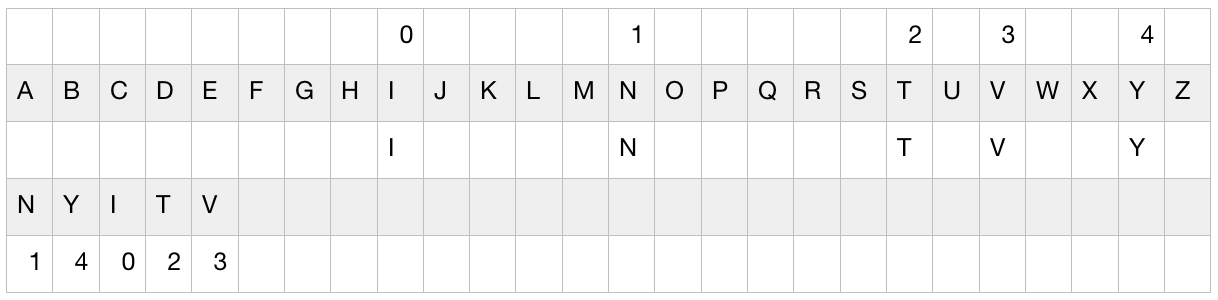
\includegraphics[scale=0.3]{./Graphs/Figure1.1.png}
  \caption{Task1-Encryption Sequence Order}
  \label{fig:testfig1}
\end{figure}



\begin{figure}[H]
  \centering
  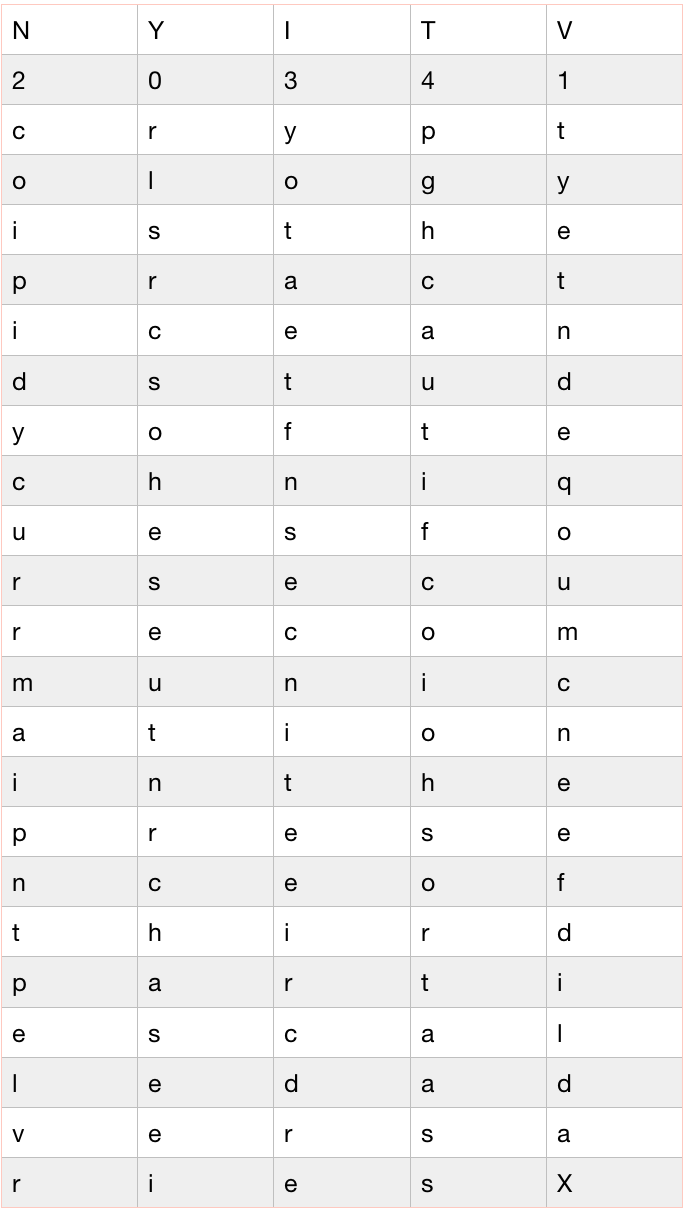
\includegraphics[scale=0.45]{./Graphs/Figure1.2.png}
  \caption{Task1-Message Matrix}
  \label{fig:testfig1}
\end{figure}
Regards for the current assignment, the empty space would be replaced by the capital letter 'X'.  Append the rows to form the ciphertext.

\begin{figure}[H]
  \centering
  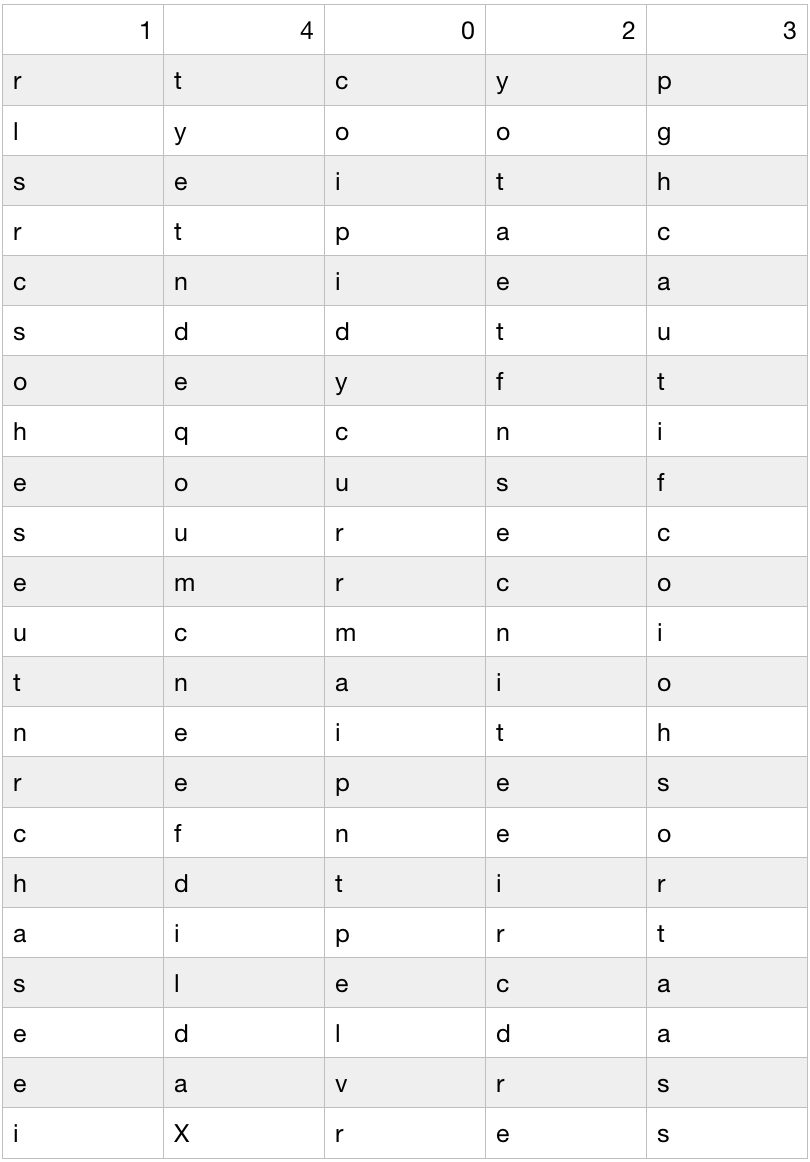
\includegraphics[scale=0.45]{./Graphs/Figure1.3.png}
  \caption{Task1-Row Transposition Matrix}
  \label{fig:testfig1}
\end{figure}

The following figure 4 displays the encrypted message.

\begin{figure}[H]
  \centering
  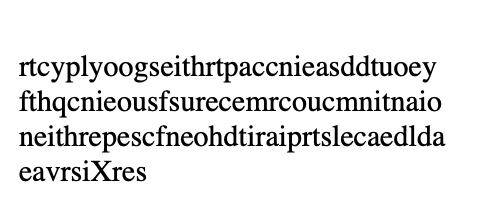
\includegraphics[scale=0.75]{./Graphs/Figure1.4.png}
  \caption{Task1-Encrypted Message}
  \label{fig:testfig1}
\end{figure}



\begin{figure}[H]
  \centering
  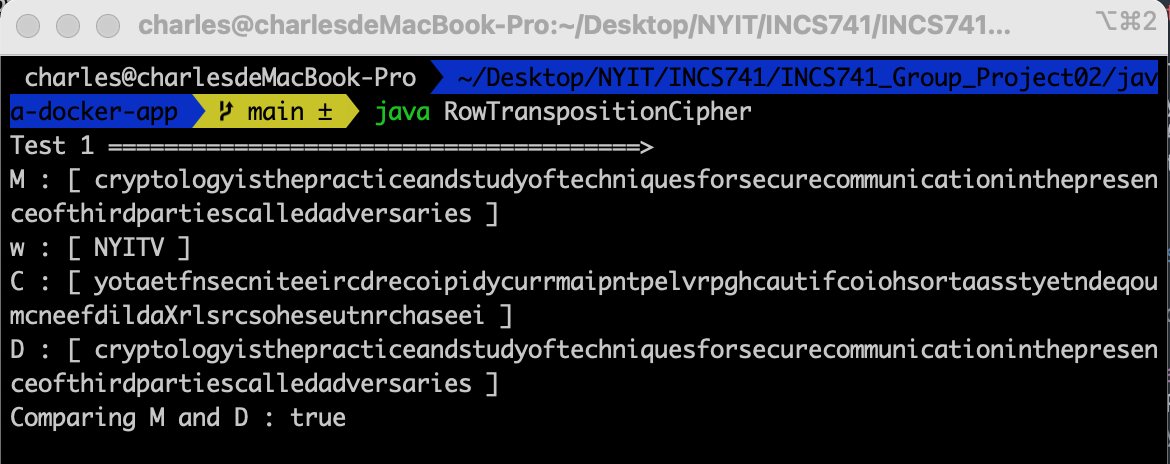
\includegraphics[scale=0.45]{./Graphs/Figure1.6.png}
  \caption{Task1-Output}
  \label{fig:testfig1}
\end{figure}

Figure 5 shows the result of the encrypted plaintext. Further, we use the decrytion algorithm to double check the answer. The result match to the original text.\\ \\ 

\vspace*{-0.35cm}
\section{Decryption Implementation}

The decryption algorithm is the reverse order of the encryption algorithm. The algorithm first writes the encrypted message out in rows. Then, it reads off the message by recording columns. \\

\begin{figure}[H]
  \centering
  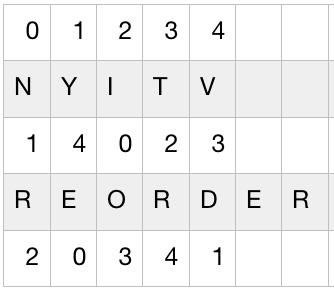
\includegraphics[scale=0.65]{./Graphs/Figure1.5.png}
  \caption{Task2-Decryption Sequence Order}
  \label{fig:testfig1}
\end{figure}

The reorder sequence is 20341 to decryption by using the same row exchange method.\\

\begin{figure}[H]
  \centering
  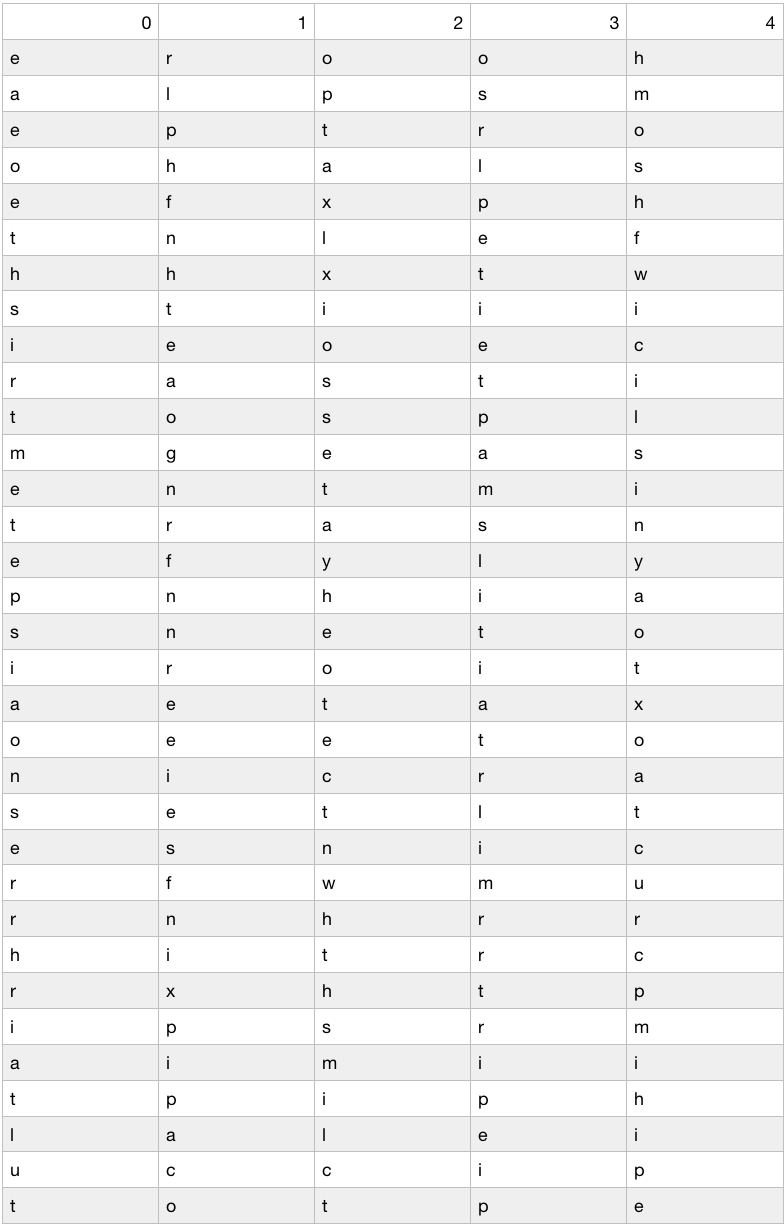
\includegraphics[scale=0.4]{./Graphs/Figure1.7.png}
  \caption{Task2-Message Matrix}
  \label{fig:testfig1}
\end{figure}

\begin{figure}[H]
  \centering
  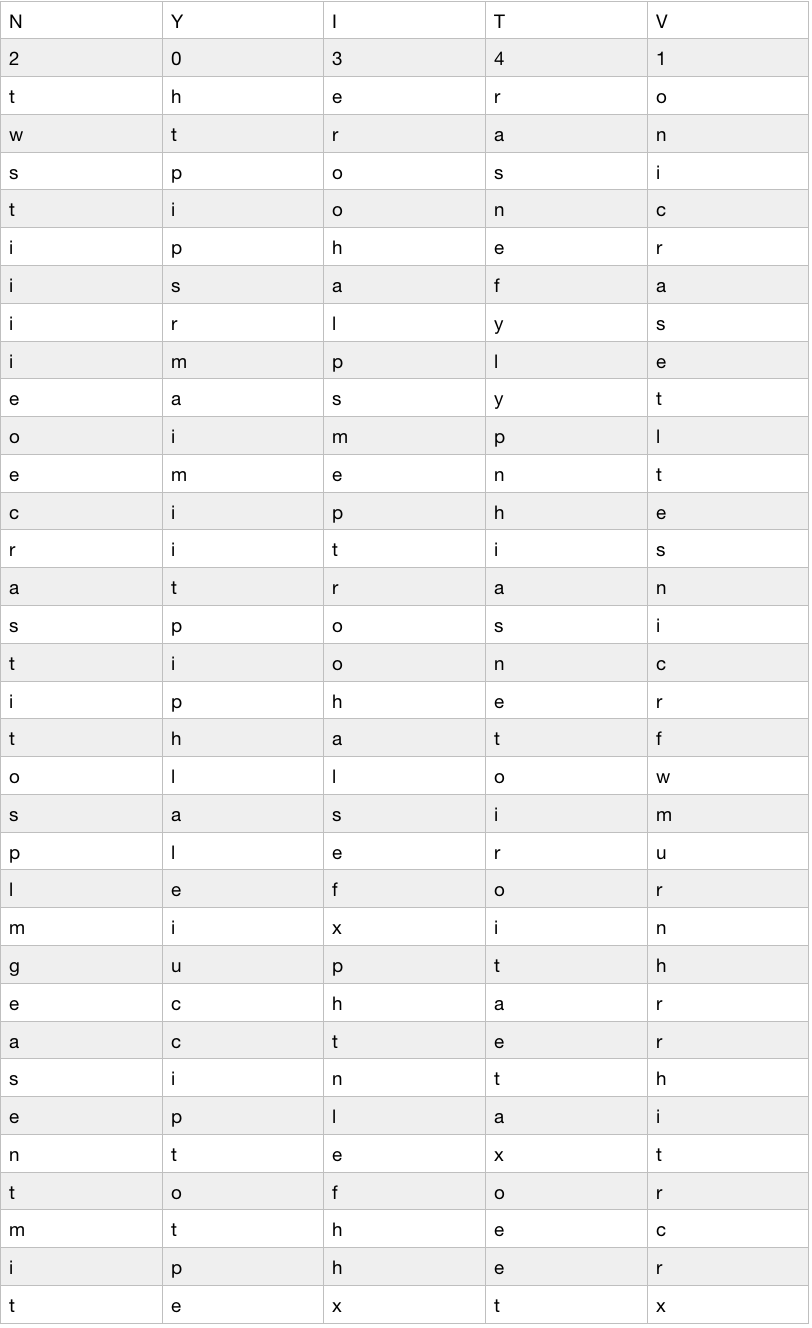
\includegraphics[scale=0.39]{./Graphs/Figure1.8.png}
  \caption{Task2-Decrypted Row Transposition Matrix }
  \label{fig:testfig1}
\end{figure}

\vspace*{0.90cm}
The first part finds the decoding sequence from the key 'NYITV'. Then, write the encrypted message into a 2D matrix 'plainTextArray'. Next, use the RowTranspositionMatrix to record the rearrangement of the 'plainTextArray'. The last step, utilize the stringbuilder to build the encrpted message line by line through the RowTranspositionMatrix.The following is the pseudocode for the row transposition cipher algorithm : \\


\floatname {algorithm} {\footnotesize Row Transposition Decryption Algorithm}
\renewcommand {\algorithmicrequire}{\textbf{input:}}
\renewcommand{\algorithmicensure}{\textbf{output:}}
\begin{algorithm}
  \caption{}\label{}
  \begin{algorithmic}[1]
  	\footnotesize
    \Require 'w' : Key and 'C' Encrypted plain-text
    \Ensure Decrypted plain-text
    \Function{rtcdecryption}{$w,C$}
      \State  $keylen \gets w.length()$
      \State $keyArray \gets key.toCharArray() $
      \State $messageArray \gets C.toCharArray() $
      \State $keyPos \gets int [keylen]$
      \State \footnotesize$ $
	  \State $Array.sort(keyArray)$
	  \State $String s \gets String.valueOf(keyArray)$	  
	  \State $keyPos \gets int [keylen]$
	  \State \footnotesize$ $
      \For{\texttt{each char c in dArray}}
        \State $keyPosition[x] \gets s.indexOf(c)$
        \State $Increament \hspace{0.1cm} x \hspace{0.1cm} by \hspace{0.1cm}1$	
      \EndFor
     
      \State \footnotesize$ $
      \State $cols \gets keylen$
      \State $rows \gets 0$
	  \If{$C's \hspace{0.1cm}length \hspace{0.1cm} mod \hspace{0.1cm} cols \hspace{0.1cm} equals \hspace{0.1cm} 0$} \Comment \tiny{calculate rows}
        \State\footnotesize $rows \gets C.length() / cols$
      \Else \Comment \tiny{calculate columns}
        \State \footnotesize$rows \gets C.length() / cols + 1$
     \EndIf
     
      \State \footnotesize$ $
      \State $plainTextArray \gets char[rows][cols]$
       
 
	  \State $k \gets 0$
	  \For{\texttt{i to rows}}
	  	\For{\texttt{j to cols}}
        	\If{$count \hspace{0.1cm}k\hspace{0.1cm} equals\hspace{0.1cm} message \hspace{0.1cm} C's \hspace{0.1cm}length$}
        	   \State $while \hspace{0.1cm} k \hspace{0.1cm} equals \hspace{0.1cm} message's \hspace{0.1cm} length \hspace{0.1cm} and \hspace{0.1cm} j \hspace{0.1cm} less \hspace{0.1cm} than \hspace{0.1cm} cols \hspace{0.1cm} keep \hspace{0.1cm} $
        	   \State $add \hspace{0.1cm}'X' \hspace{0.1cm} to \hspace{0.1cm} plainTextArray[i][j]$
        	   \State $break$
        	   \State \tiny$plainTextArray[i][j] \gets messageArray[k]$
        	   \State \footnotesize $Increament\hspace{0.1cm} k\hspace{0.1cm} by \hspace{0.1cm}1$	
        	   \State \footnotesize$ $
		    \EndIf
        \EndFor  
      \EndFor  
         
      \State  $rowTranspositionMatrix \gets char[rows][cols] $
      \For{\texttt{i to rows}}
	  	\For{\texttt{j to cols}} \Comment \tiny{each column read by the key order}
	  		\State \tiny$RowTranspositionMatrix[i][j]  \gets plainTextArray[i][keyPosition[j]]$  
        \EndFor  
      \EndFor    
      
      \State \footnotesize$ $
      
      \State \footnotesize $ StringBuilder\hspace{0.1cm} str \gets StringBuilder()$
      \For{\texttt{i to rows}}
	  	\For{\texttt{j to cols}}
        	\State $str.append(RowTranspositionMatrix[i][j])$   	
        \EndFor  
      \EndFor  
      
      \State \textbf{return} $str$\Comment \tiny{Decrypted message is str}
    \EndFunction
  \end{algorithmic}
\end{algorithm}




\begin{figure}[H]
  \centering
  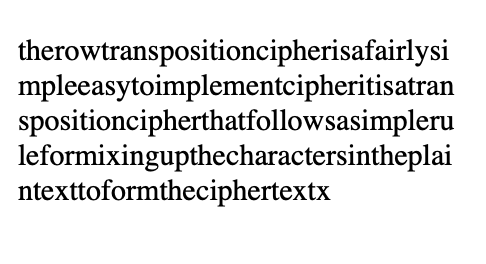
\includegraphics[scale=0.75]{./Graphs/Figure1.9.png}
  \caption{Task2-Decrypted Message}
  \label{fig:testfig1}
\end{figure}
\begin{figure}[H]
  \centering
  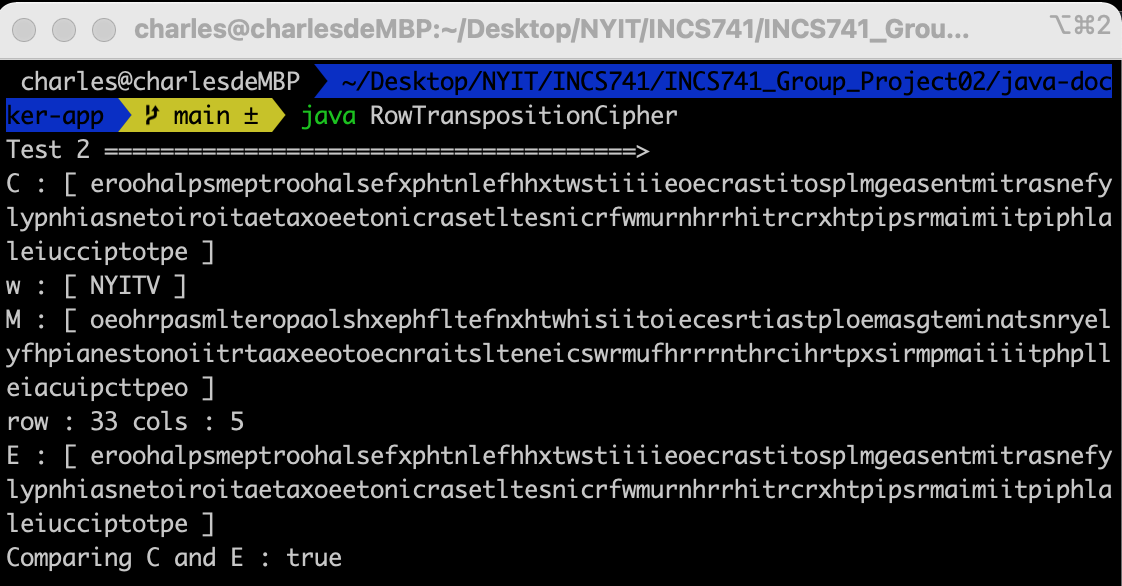
\includegraphics[scale=0.36]{./Graphs/Figure2.0.png}
  \caption{Task2-Output}
  \label{fig:testfig1}
\end{figure}

Figure 10 shows the result of the decrypted plaintext. Further, we use the encrytion algorithm to double check the answer. The result match to the original encrypted text.

\section{Conclusion}

With the growing use of computers and the Internet, and an increasing need to transmit information quickly and securely, the use of encryption through existing protocols (AES, RSA, 3DES, etc.) information security that uses the two types of transposition mentioned (transposition and substitution).

In this example, we can see that using only one round of encryption and a minor key (5 letters), the information is already quite challenging to decipher, and with the use of the protocols mentioned above that repeatedly use the types of transposition, it becomes almost impossible to decipher the messages.

We also demonstrate in the project that the information is decrypted, just doing the inverse of the encryption procedure that needs to be done by the person who will receive the message. \\ 

%----------------------------------------------------------------------------------------
%	REFERENCE LIST
%----------------------------------------------------------------------------------------
\begin{thebibliography}{} % Bibliography - this is intentionally simple in this template
\footnotesize[1]G. Newell, “An introduction to linux access control lists (acls),” Enable Sysadmin, 07-Jan-2022. [Online]. Available: https://www.redhat.com/sysadmin/linux-access-control-lists. [Accessed: 21-Feb-2022]. \\ \\
 
\end{thebibliography}


%----------------------------------------------------------------------------------------

\end{document}
